\chapter{ Технологический раздел}
\label{cha:technological}

    В данном разделе будут выбраны средства реализации ПО и представлен листинг кода. 

    \section{Средства реализации}
        В данной работе используется язык программирования C\# \cite{c-sharp}, так как
        он позволяет написать программу в относительно малый срок.
        В качестве среды разработки использовалась Visual Studio Code \cite{binary-search}. 

    \section{Листинг программы}
        Ниже представлены листинги кода алгоритмов:
        \begin{enumerate}
            \item полного перебора (листинг \ref{lst:brute-force});
            \item муравьиного (листинг \ref{lst:ant}).
        \end{enumerate}
        
        \begin{lstlisting}[language={[Sharp]C}, label=lst:brute-force, caption=Реализация алгоритма поиска полным перебором]
public class BruteForceAlgorithm : IRouteAlgorithm
{
    public Path GetRoute(Map map)
    {
        Path shortest = new Path(null, map);
        foreach (var cur in GetAllRoutes(map.N))
        {
            cur.Add(0);
            Path check = new Path(cur, map);
            if (shortest.Distance > check.Distance)
                shortest = check;
        }
        return shortest;
    }

    private IEnumerable<List<int>> GetAllRoutes(int count)
    {
        List<int> cur = new List<int>();
        for (int i = 0; i < count; i++)
            cur.Add(i);

        while (NextSet(cur, count))
            yield return new List<int>(cur);
    }

    private bool NextSet(List<int> cur, int count)
    {
        int j = count - 2;
        while (j != -1 && cur[j] >= cur[j + 1]) 
            j--;

        if (j == -1 || cur[j] == 0)
            return false;

        int k = count - 1;
        while (cur[j] >= cur[k])
            k--;
        Swap(cur, j, k);
        int left = j + 1;
        int right = count - 1;

        while (left < right)
            Swap(cur, left++, right--);
        return true;
    }

    private void Swap(List<int> cur, int i, int j)
    {
        int tmp = cur[i];
        cur[i] = cur[j];
        cur[j] = tmp;
    }
}
        \end{lstlisting}

        \begin{lstlisting}[language={[Sharp]C}, label=lst:ant, caption=Реализация муравьиного алгоритма]
public class AntsAlgorithm : IRouteAlgorithm
{
    public AntsAlgorithm(int maxTime, double alpha, double beta, double q, double pho)
    {
        MaxTime = maxTime;
        Alpha = alpha;
        Beta = beta;
        Q = q;
        Pho = pho;
    }

    public int MaxTime { get; set; }
    public double Alpha { get; set; }
    public double Beta { get; set; }
    public double Q { get; set; }
    public double Pho { get; set; }


    public Path GetRoute(Map map)
    {
        Random r = new Random();
        Path shortest = new Path(null, map);

        int count = map.N;
        double[,] pher = InitPheromone(0.1, count);

        for (int time = 0; time < MaxTime; time++)
        {
            var ants = InitAnts(map);
            for (int i = 0; i < count - 1; i++)
            {
                double[,] deltaPher = InitPheromone(0, count);
                foreach (var ant in ants)
                {
                    int curTown = ant.LastVisited();

                    double sum = 0;
                    for (int town = 0; town < count; town++)
                    {
                        if (!ant.IsVisited(town))
                        {
                            double tau = pher[curTown, town];
                            double eta = 1 / map[curTown, town];
                            sum += Math.Pow(tau, Alpha) * Math.Pow(eta, Beta);
                        }
                    }

                    double check = r.NextDouble();
                    int newTown = 0;
                    for (; check > 0; newTown++)
                    {
                        if (!ant.IsVisited(newTown))
                        {
                            double tau = pher[curTown, newTown];
                            double eta = 1 / map[curTown, newTown];
                            double chance = Math.Pow(tau, Alpha) * Math.Pow(eta, Beta) / sum;
                            check -= chance;
                        }
                    }
                    newTown--;
                    ant.VisitTown(newTown);
                    deltaPher[curTown, newTown] += Q / map[curTown, newTown];
                }
                for (int k = 0; k < count; k++)
                    for (int t = 0; t < count; t++)
                        pher[k, t] = (1 - Pho) * pher[k, t] + deltaPher[k, t];
            }
            foreach (var ant in ants)
            {
                ant.VisitTown(ant.Start);
                if (ant.GetDistance() < shortest.Distance)
                    shortest = ant.Path;
            }
        }

        return shortest;
    }

    private List<Ant> InitAnts(Map map)
    {
        var ants = new List<Ant>(map.N);
        for (int i = 0; i < map.N; i++)
            ants.Add(new Ant(map, i));
        return ants;
    }

    private double[,] InitPheromone(double num, int size)
    {
        double[,] phen = new double[size, size];
        for (int i = 0; i < size; i++)
            for (int j = 0; j < size; j++)
                phen[i, j] = num;
        return phen;
    }
}
        \end{lstlisting}
    
        
    \section{Тестирование}
        В таблице \ref{table:testing} отображён возможный набор тестов
        для тестирования методом чёрного ящика, результаты которого, 
        представленные на рисунке \ref{png:testing:result}, подтверждают
        прохождение программы перечисленных тестов.
        
        \begin{table}[]
            \caption{Тесты для проверки корректности программы}
            
            \centering
            \begin{tabular}{|c|c|}
            \hline
            Матрица смежности                                                                                    & \begin{tabular}[c]{@{}c@{}}Минимальное\\ расстояние\end{tabular} \\ \hline
            $\begin{bmatrix} 0 & 10\\ 10 & 0 \end{bmatrix}$                                                      & 20                                                               \\ \hline
            $\begin{bmatrix}0 & 10 & 15 & 20\\10 & 0 & 35 & 25\\15 & 35 & 0 & 30\\20 & 25 & 30 & 0\end{bmatrix}$ & 80                                                               \\ \hline
            \end{tabular}
            \label{table:testing}
        \end{table}

        \begin{figure}[h!]
            \centering
            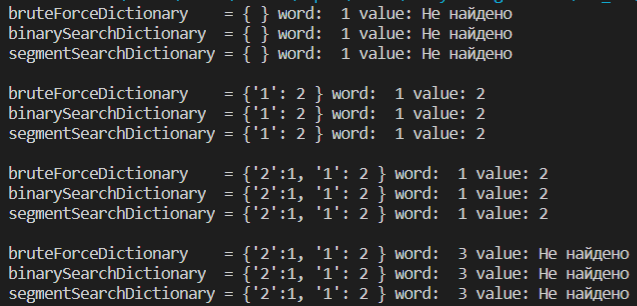
\includegraphics[scale=0.9]{testing.png}
            \caption{Результаты тестирования алгоритмов.}
            \label{png:testing:result}
        \end{figure}
\newpage